\tias{to whoever is proofreading the paper: check for consistency: reasoning step or inference step?}

% Based on 'explaining explanations' paper: interpretable and complete; interpr: understandable to humans, simple enough using voca that is meaningful to user; explanation-producing systems;

%Compute explanation of form C /\ B -> A. By find B = MUS(not A, C) so not a and C and B so a <- B and C; BnC may generate more, so apply BnC to obtain A and B and C -> A. (This is why 'B' and nr of constraints C have to be small);
%Simplicity: size of B, C and A as small as possible, 

%Need for explanations of reasoning systems
Explainable AI research aims to fulfill the need for trustworthy AI systems that can explain their reasoning in a human-understandable way. 
As these systems employ more advanced reasoning mechanisms and computation power, it becomes increasingly difficult to understand why certain decisions are made. 
Understanding the decisions is important for verifying the correctness of the system, as well as to control for biased or systematically unfair decisions.

Explainable AI is often studied in the context of (black box) machine learning systems such as neural networks, where the goal is to provide insight into what part of the input is important in the \textit{learned} model. These insights (or local approximations thereof) can justify why certain predictions are made. In contrast, in constraint satisfaction problems, the problem specification is an explicit model-based representation of the problem, hence creating the opportunity to explain the inference steps directly in terms of this representation.
%Another domain is explainable planning, which looks among others at answering user queries regarding a computed plan and model reconciliation.\bart{Beetje kort. Kan je daar meer over zeggen? }

%Shallow related work on quickxplain, 'explanations' in search, etc.
Explanations have been investigated as part of constraint solving before, most notably for explaining over-constrained, and hence unsatisfiable, problems to a user~\cite{junker2001quickxplain}. Our case is more general in that it also works for satisfiable problems. At the solving level, in lazy clause generation solvers, explanations of a constraint are studied in the form of an implication of low-level Boolean literals that encode the result of a propagation step of an individual constraint~\cite{feydy2009lazy}. Also, nogoods (learned clauses) in conflict-driven clause learning SAT solvers can be seen as explanations of failure during search~\cite{marques2009conflict}. These are not meant to be human-interpretable but rather to propagate efficiently.
%BART: replaced nogoods (unsat cores) by nogoods (learned clauses) 


We aim to explain the process of propagation in a constraint solver, independent of the consistency level of the propagation and without augmenting the propagators with explanation capabilities.
For problems that can --- given a strong enough propagation mechanism --- be solved without search, e.g. problems such as logic grid puzzles with a unique solution, this means providing an explanation of the entire problem solving process. For problems involving search, this means explaining the inference steps taken within one search node. 
It deserves to be stressed that we are not interested in the computational cost of performing an expensive form of propagation, but rather in explaining all consequences of a given assignment to the user in a way that is as understandable as possible. 
% \bart{Generalized Arc Consistency is toch niet helemaal hetzelfde als optimalpropagate...} % optimalpropagate is volgens mij nog sterker. GAC kijkt nog altijd constraint per constraint. optimalpropagate doet een soort global propagation over alle constraints heen. Is GAC over een nieuwe constraint die de unie van alle andere is. Ik heb bovenstaande paragraaf nog wat uitgebreid. Ook in onderstaande paragraaf nog wat aangepast. Specifiek de zin ``e.g. none of the constraints can be used to derive new facts'' weggehaald want dat suggereert dat elke constraint apart propageert terwijl het bij ons juist essentieel dat combinaties mogelijk zijn (bijv tussen clue en bijectivities)}
% \tias{IDD, optimal propagate is eerder 'global consistency'. Ik vind geen definitie, maar basically globally consistent = voldoet aan alle constraints, e.g. kan uitgebreid worden naar een oplossing zonder dat over deze variabele moet gebacktracked worden = de unie van alle mogelijke oplossingen}

More specifically, we aim to develop an explanation-producing system that is complete and interpretable. By \textit{complete} we mean that it finds a \textit{sequence} of small reasoning steps that, starting from the given problem specification and a partial solution, leads to the partial solution obtained when propagating until fixed-point (i.e., all consequences of the current assignment are derived). %An explanation of one reasoning step is an implication of the form $E \wedge S \rightarrow N$, where $E$ is \textit{evidence} namely a (sub)set of previously derived facts, $S$ is a (sub)set of constraints, and $N$ is a set of newly derived facts that follow from $E$ and $S$.
%
Gilpin et al.~\cite{DBLP:conf/dsaa/GilpinBYBSK18} define \textit{interpretable} explanations as ``descriptions that are simple enough for a person to understand, using a vocabulary that is meaningful to the user''. Our guiding principle is hence that of simplicity, where smaller and simpler explanations are better. %$E \wedge S \rightarrow N$ 
We choose to represent the constraints in natural language, which is an obvious choice for logic grid puzzles where they are given as natural language \textit{clues} in the first place. For representing the previously and newly derived facts, we use a visualisation in the solution structure, as can be seen in the grid in Figure~\ref{fig:zebrascreen}.

%HolyGrail challenge and related work
Our work is motivated by Eugene Freuder's ``Holy Grail Challenge''\footnote{\tiny \url{https://freuder.wordpress.com/pthg-19-the- third-workshop-on-progress-towards-the-holy-grail/}} which had as objective to provide automated processing of logic grid puzzles, ranging from natural language processing, to solving, and explanining. 
An earlier version of our system was the challenge winner at the workshop. 
%There has been previous work on automatically \emph{solving} logic grid puzzles, starting from the natural language clues \cite{related,work}\tias{TODO}. 
While our system also has the capability of solving logic grid puzzle starting from the natural language clues (see Section \ref{sec:holistic}), the focus of this paper is on the novel explanation-producing part of the system.

The explanation-generating techniques we develop can be applied in a multitude of use cases. 
For instance, our tool can explain the entire sequence of reasoning, such that a user can debug either the reasoning system or the set of constraints that are given as problem specification. 
As our approach starts from an arbitrary set of facts, it can also be used as a virtual assistant when a user is stuck in solving a problem, where the system will explain the simplest possible next move, or in an interactive setting where a system can explain how it would complete a partial solution of a user.
Finally, our measures of simplicity of reasoning steps can be used to estimate the difficulty of solving a problem for a human, e.g. for gradual training of experts.

%challenge 1: abstraction in self-contained reasoning step
%challenge 2: ordering
%challenge 3: computation efficiency
%The challenge in making an explanation-producing constraint solving method is choosing the right level of abstraction for the constraints and explanations, defining what a good ordering of the explanations is, and extracting a complete sequence of good explanations in a computationally efficient way. The search for a sequence of small explanations is much more computationally intensive than searching for a satisfying solution as it requires repeatedly solving subparts of the problem.

%Contributions: (eerste aanzet!!!)
\noindent Our contributions are the following:
\begin{compactitem}
	\item We formalize the problem of step-wise explaining the propagation of a constraint solver through a sequence of small inference steps;
	\item We propose an algorithm that is agnostic to the propagators and the consistency level used, and that can provide explanations for inference steps involving arbitrary combinations of constraints;
	\item Given a cost function quantifying interpretability, our method uses an optimistic estimate of this function to guide the search to low-cost explanations, thereby making use of Minimal Unsatisfiable Subset extraction;
	\item We experimentally demonstrate the quality and feasibility of the approach in the domain of logic grid puzzles.
\end{compactitem}
%\bart{``that are Minimal Unsatisfiable Subsets of constraints and previously derived facts;'' is not really correct. Since these would be consistent. The negated part is important. Replaced with ``thereby building on top of Minimal Unsatisfiable Subset algorithms'' } Ack
\ 

The paper is organized as follows: we first discuss related work and background knowledge on logic grid puzzles and first-order logic based constraint solving. We then define the problem, after which we explain our proposed algorithm. Next, we explain the instantiation of our algorithm for logic grid puzzles and how this fits in an end-to-end solution that starts from the natural language clues, followed by experiments and conclusions.
%\bart{if space permits :p I don't find this neccesary for a 7page paper}


\begin{figure}[t]
\centering
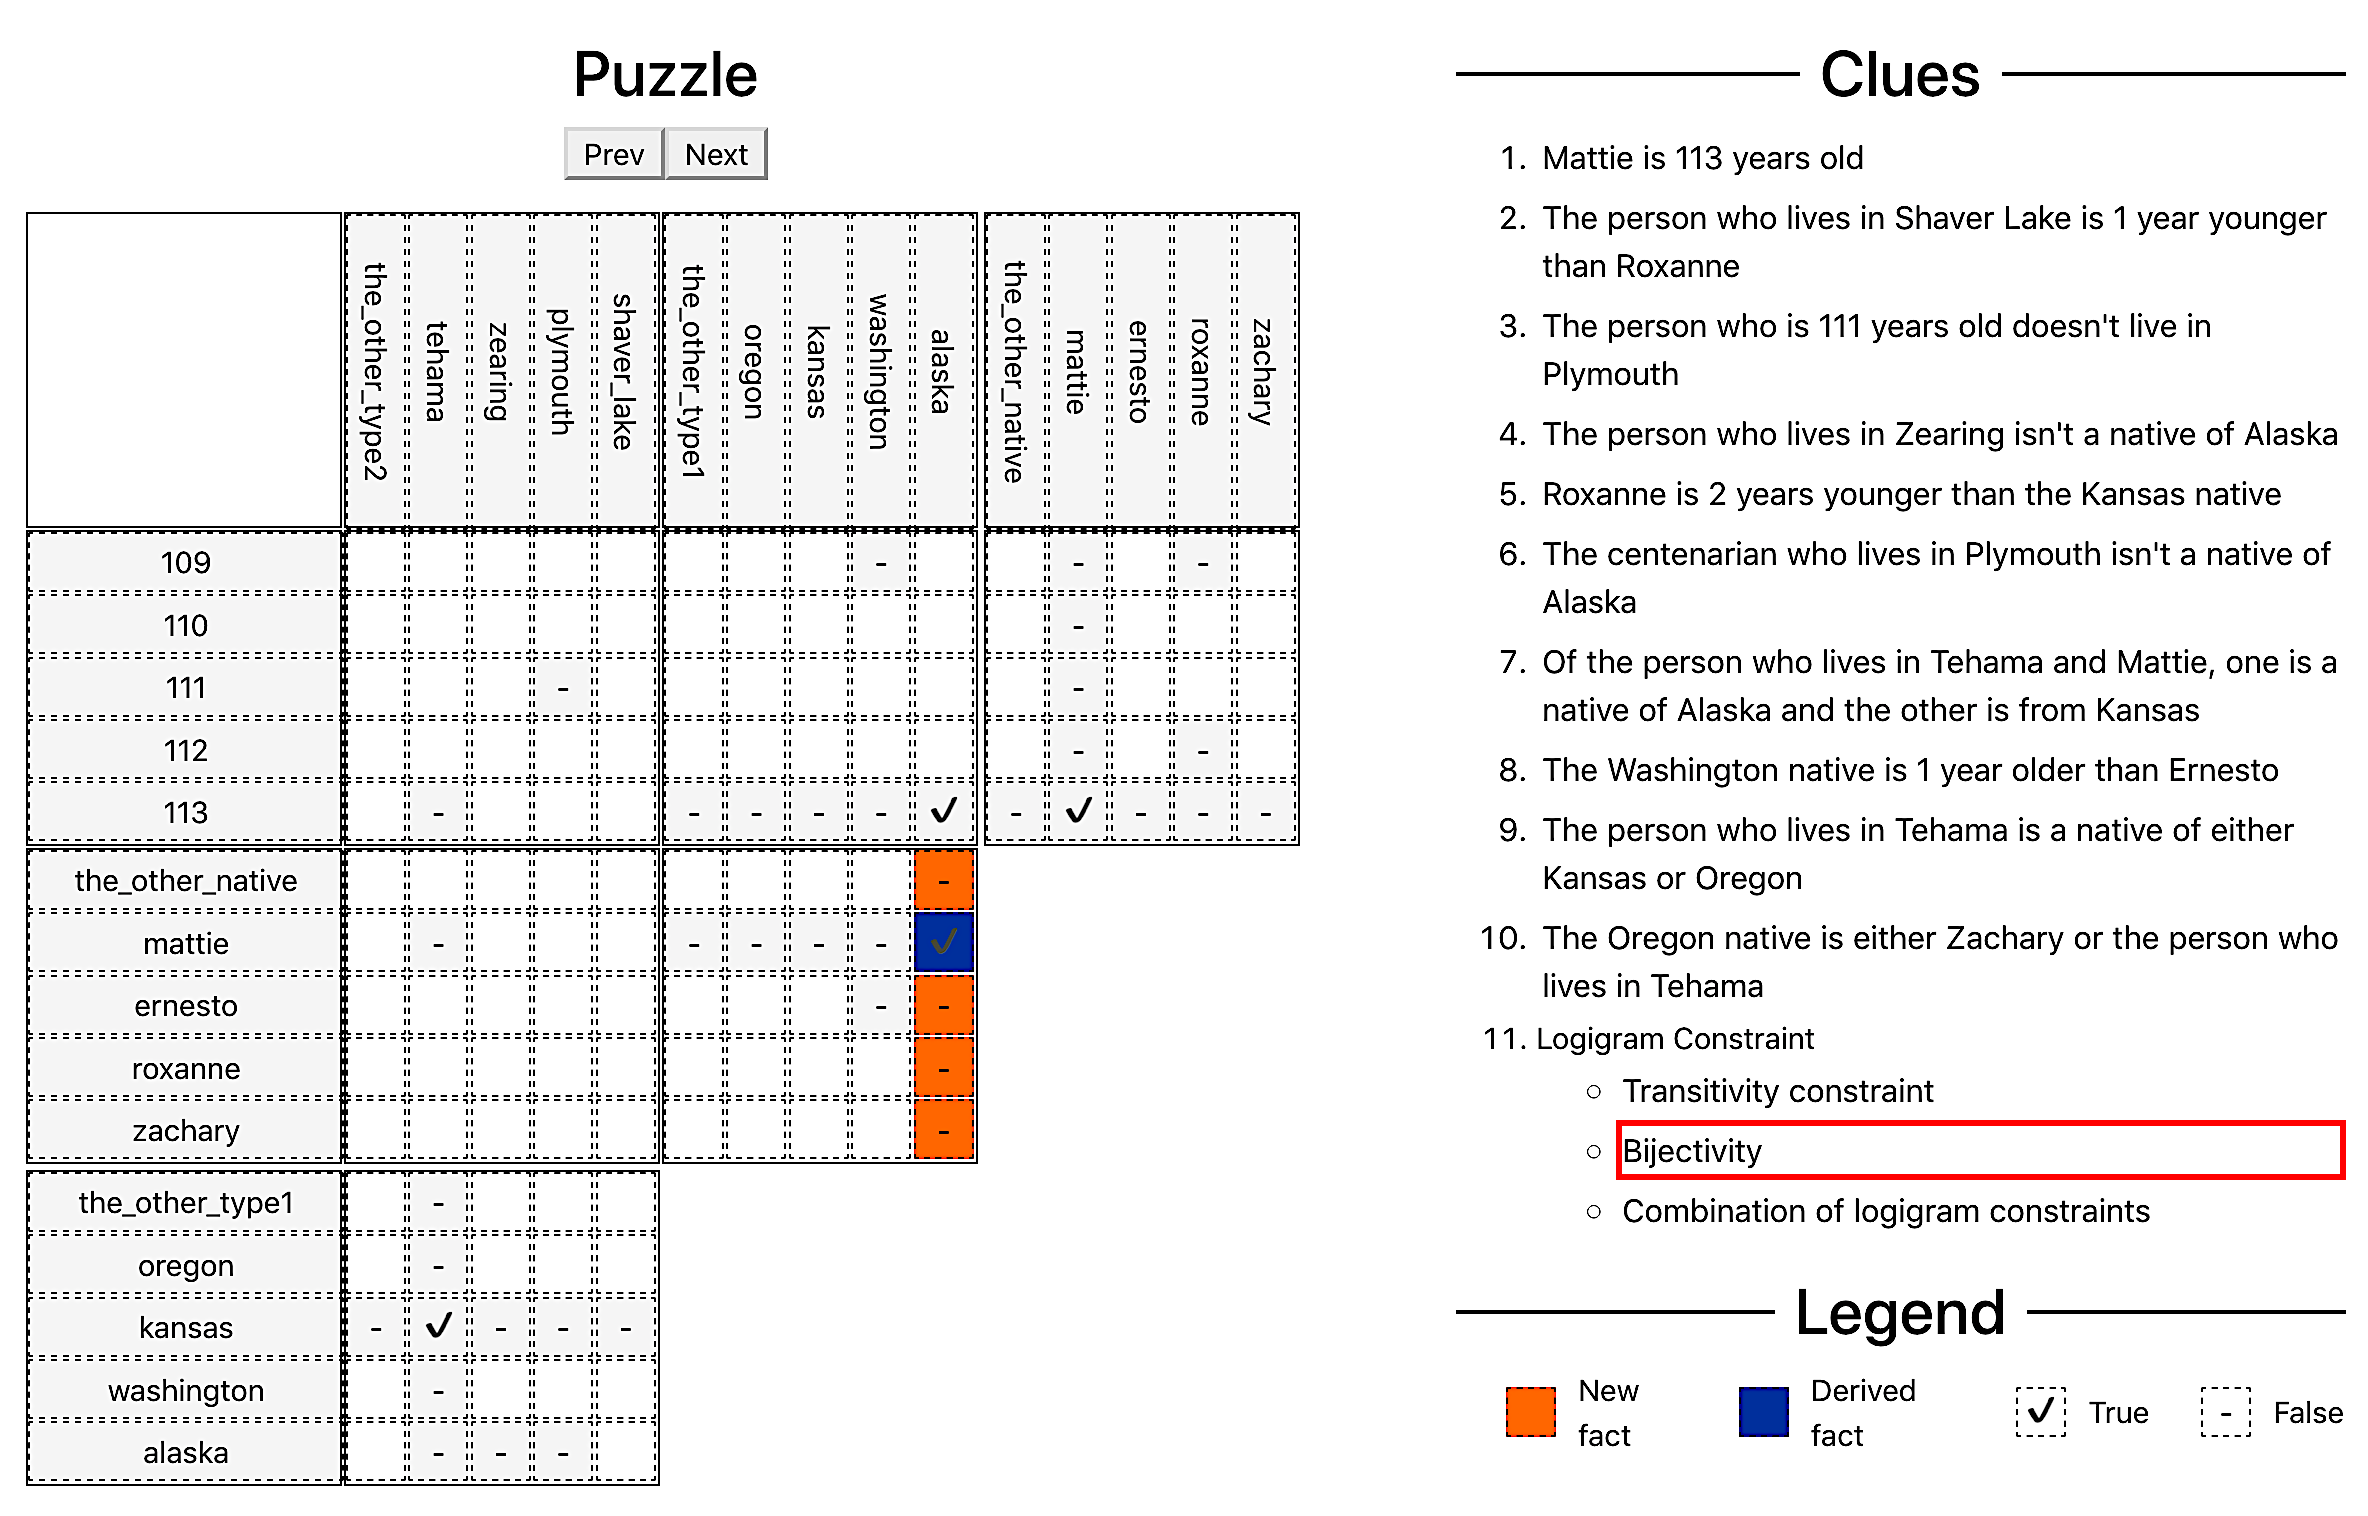
\includegraphics[width=1\linewidth]{zebra_screen}
\caption{Demonstration of explanation visualisation.}
\label{fig:zebrascreen}
\end{figure}

